\chapter{Planificaci\'on}

\section{Metodolog\'ia utilizada}
Para el desarrollo de esta app, usar\'e una metodolog\'ia \textit{\'agil} tipo \textbf{SCRUM}. He decidido usar esta porque me permite corregir fallos en la velocidad de dise\~no y/o planificaci\'on de forma eficiente y sin da\~nar el producto final.

Las reuniones con la tutora ser\'an las \textit{sprint reviews}.

\section{Temporizaci\'on}
La temporizaci\'on se realiz\'o el d\'ia 25 de marzo de 2025. La entrega del producto (este TFG) est\'a prevista para el 16 de junio de 2025, es decir, 83 d\'ias, o lo que es lo mismo, casi 12 semanas. Si un sprint dura 2 semanas, habr\'a 6 sprints hasta la entrega final.

La iteraci\'on 0 se dedicar\'a al dise\~no de pantallas y al repaso de las funcionalidades de la app. La idea inicial es dividir la app en varios m\'odulos y centrar cada sprint en uno de ellos:

\begin{itemize}
  \item Diagramas de la app y ejercicios
  \item Rutinas, usuarios y sesi\'on
  \item Datos que ingresa el usuario
  \item Flujo de entrenamiento
  \item Inteligencia Artificial (IA)
  \item Smartwatch
\end{itemize}

\section{Seguimiento del desarrollo}

\subsection*{Iteraci\'on 0}
En esta primera iteraci\'on me cent\'re en completar los dise\~nos de la app, priorizando su accesibilidad. Tambi\'en concret\'e el \textit{product backlog}, compuesto por 25 historias de usuario. Algunas incluyen tareas secundarias:

\begin{description}
  \item[\textbf{SCRUM-1}] Registrar peso por d\'ia
  \item[\textbf{SCRUM-2}] Establecer peso objetivo
  \item[\textbf{SCRUM-3}] Insertar/Borrar/Modificar ejercicio de la lista
  \item[\textbf{SCRUM-4}] Buscar rutina en la lista del usuario
  \item[\textbf{SCRUM-5}] Sustituir un ejercicio por otro en la rutina
  \item[\textbf{SCRUM-6}] Insertar/Borrar/Modificar rutina
  \item[\textbf{SCRUM-7}] Poner una meta en cada ejercicio
  \item[\textbf{SCRUM-8}] Graficar los datos de los ejercicios
  \item[\textbf{SCRUM-9}] Revisar datos para ver si el descanso es necesario
  \item[\textbf{SCRUM-10}] Ense\~nar datos de una rutina a descargar
  \item[\textbf{SCRUM-11}] Compartir mi rutina
  \item[\textbf{SCRUM-12}] Guardar las repeticiones y series de todos los ejercicios de un entrenamiento
  \item[\textbf{SCRUM-13}] Valorar el entrenamiento en base a la marca actual y la meta del usuario
  \item[\textbf{SCRUM-14}] Monitorizar pulso en tiempo real
  \item[\textbf{SCRUM-15}] Medir pulso en reposo y compararlo con datos de ejercicios
  \item[\textbf{SCRUM-16}] Avisar de anomal\'ias en el pulso de forma suave
  \item[\textbf{SCRUM-17}] Obtener calor\'ias quemadas
  \item[\textbf{SCRUM-18}] Comprobar el equilibrio nervioso del usuario
  \item[\textbf{SCRUM-19}] Ejecutar el flujo del entrenamiento
  \item[\textbf{SCRUM-20}] Conectar con la IA para iniciar di\'alogo
  \item[\textbf{SCRUM-21}] Crear/Borrar usuario
  \item[\textbf{SCRUM-22}] Resumir datos
  \item[\textbf{SCRUM-23}] Iniciar/Cerrar sesi\'on
  \item[\textbf{SCRUM-24}] Medir SpO2
  \item[\textbf{SCRUM-25}] Interpretar constantes
\end{description}

A continuación se muestran los diseños creados en esta iteración:

\begin{figure}[H]
  \centering
  \begin{minipage}[b]{0.6\textwidth}
    \centering
    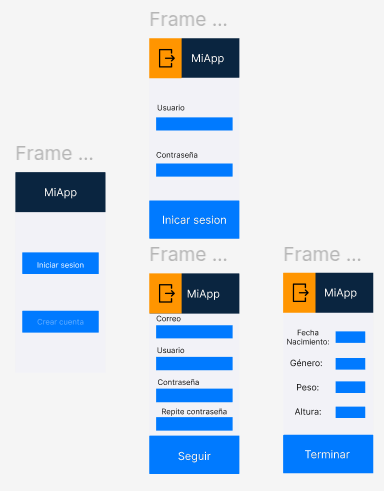
\includegraphics[width=\textwidth]{fotos/Init.png}
    \caption{Pantalla inicial}
    \label{fig:Pantalla inicial}
  \end{minipage}
  \hfill
  \begin{minipage}[b]{0.35\textwidth}
    \centering
    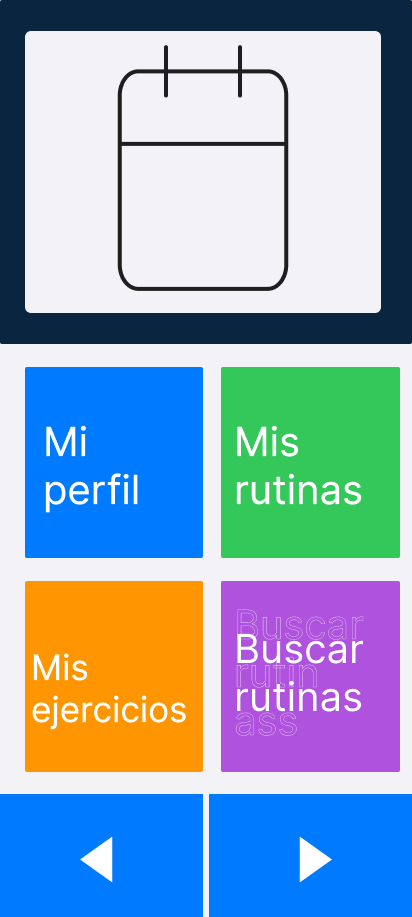
\includegraphics[width=\textwidth]{fotos/MainMenu.png}
    \caption{Menú principal}
    \label{fig:Menu principal}
  \end{minipage}
  \begin{minipage}[b]{0.45\textwidth}
    \centering
    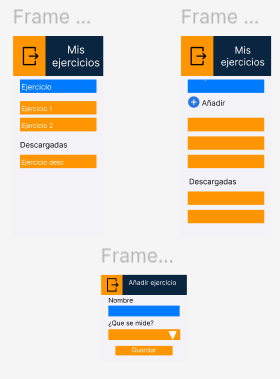
\includegraphics[width=\textwidth]{fotos/ListaEjercicios.png}
    \caption{Lista ejercicios}
    \label{fig:Lista ejercicios}
  \end{minipage}
  \begin{minipage}[b]{0.45\textwidth}
    \centering
    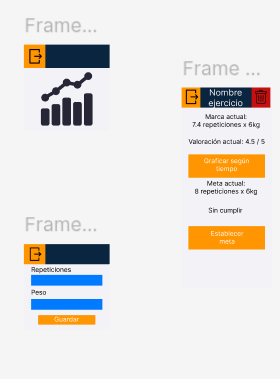
\includegraphics[width=\textwidth]{fotos/DatosEjercicios.png}
    \caption{Datos ejercicios}
    \label{fig:Datos ejericicios}
  \end{minipage}
\end{figure}


\clearpage

\subsubsection*{Sprint Review 0}
Durante esta revisi\'on de sprint se realizaron mejoras de dise\~no, como la incorporaci\'on de iconos en todos los botones para mejorar la accesibilidad. Se revisaron los t\'itulos de las ventanas, cambiando aquellos que no eran lo suficientemente claros.

Adem\'as, se a\~nadieron nuevas historias al \textit{product backlog}:

\begin{itemize}
  \item Copiar rutina
  \item A\~nadir meta por par\'ametro
  \item Solicitar permiso al usuario antes de enviar datos a la IA
  \item Enviar datos del entrenamiento actual y anteriores a la IA
  \item Conectar/Desconectar con la IA
\end{itemize}

\subsection*{Iteraci\'on 1}
Al inicio de esta iteraci\'on detect\'e la ausencia de historias para el dise\~no de diagramas de la app y la base de datos. Por ello, se a\~nadi\'o la siguiente historia:

\begin{description}
  \item[\textbf{SCRUM-26}] Dise\~nar las tablas de la base de datos
\end{description}

\begin{figure}[h!]
  \centering
  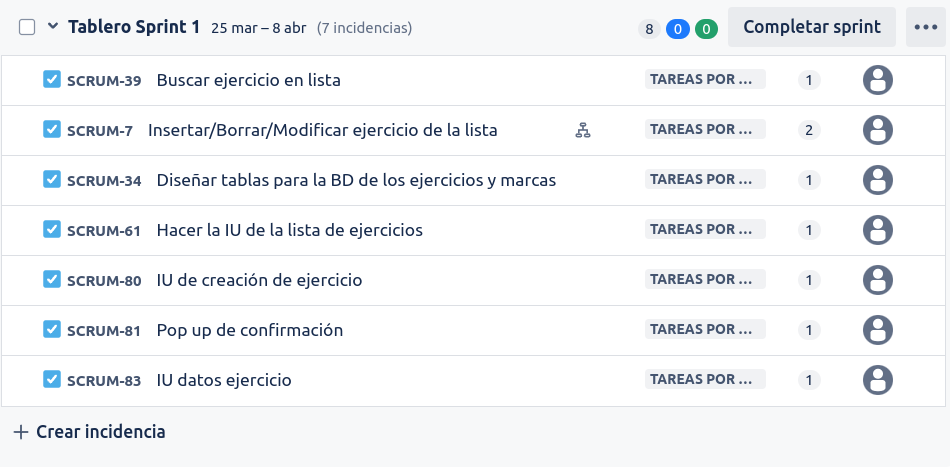
\includegraphics[width=0.7\textwidth]{fotos/PreSrprint1.png}
  \caption{Planificaci\'on Sprint 1}
  \label{fig:pre_sprint1}
\end{figure}

\begin{figure}[h!]
  \centering
  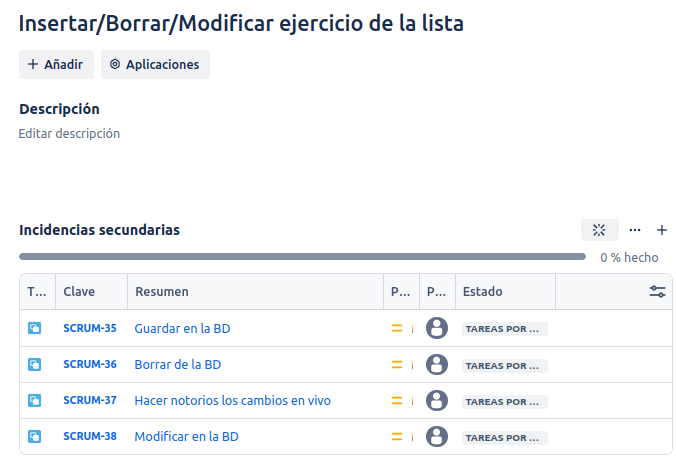
\includegraphics[width=0.7\textwidth]{fotos/SubListPre1.png}
  \caption{Subtareas Sprint 1}
  \label{fig:sublist_pre1}
\end{figure}

Durante esta iteraci\'on me familiaric\'e con Flutter y sus herramientas, como la base de datos local \textit{SQLite}.

\subsubsection*{SQLite}
Es una base de datos ligera, autocontenida y de c\'odigo abierto. Usa el mismo lenguaje de consultas que SQL, lo que la hace ideal para la app. Adem\'as, permite transportar toda la BD en un \textit{.db}, lo cual puede facilitar funcionalidades como copias de seguridad descargables desde la nube.

\subsubsection*{Sprint Review 1}
Las primeras iteraciones tienden a ser m\'as lentas debido a la fase inicial del desarrollo. No se complet\'o la totalidad del sprint; qued\'o pendiente la subtarea de modificar ejercicio en la base de datos. Aun as\'i, las expectativas son positivas, ya que se espera un aumento en la velocidad de desarrollo. No obstante, en lo que se lleva  desarrollado han aparecido pocas problemáticas

\begin{figure}[h!]
  \centering
  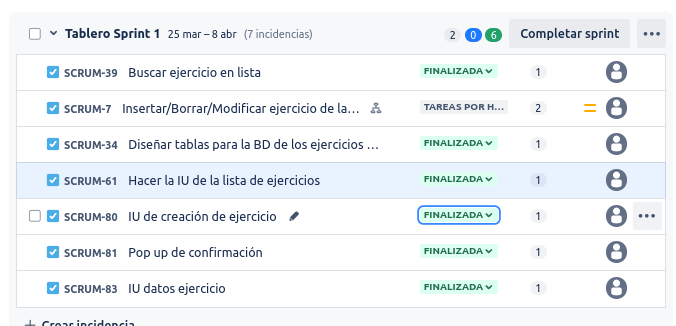
\includegraphics[width=0.7\textwidth]{fotos/PostSprint1.png}
  \caption{Fin Sprint 1}
  \label{fig:post_sprint1}
\end{figure}

\begin{figure}[h!]
  \centering
  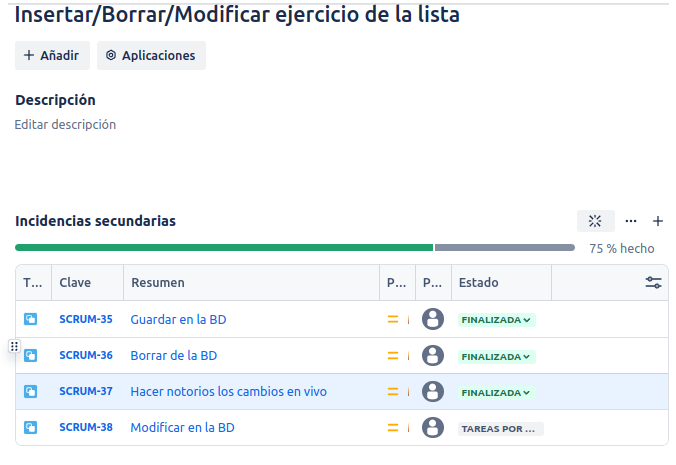
\includegraphics[width=0.7\textwidth]{fotos/SubListPost1.png}
  \caption{Subtareas completadas Sprint 1}
  \label{fig:sublist_post1}
\end{figure}

\begin{figure}[h!]
  \centering
  \begin{minipage}[b]{0.45\textwidth}
    \centering
    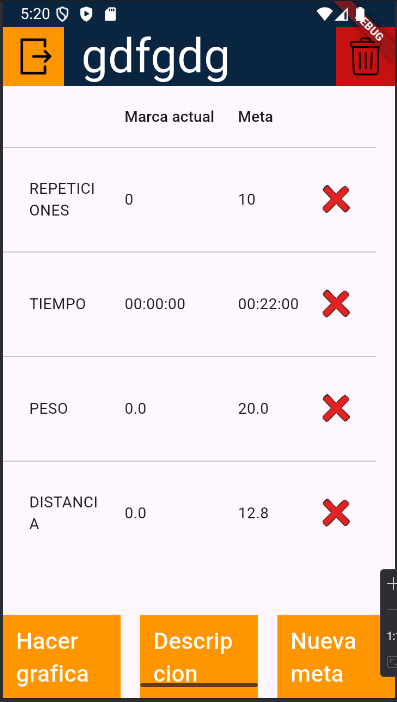
\includegraphics[width=\textwidth]{fotos/ejerciciosNueva.png}
    \caption{Pantalla nueva}
    \label{fig:pantalla_nueva}
  \end{minipage}
  \hfill
  \begin{minipage}[b]{0.45\textwidth}
    \centering
    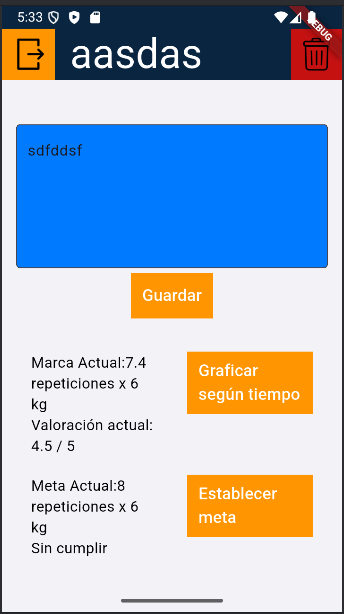
\includegraphics[width=\textwidth]{fotos/ejerciciosVieja.png}
    \caption{Pantalla antigua}
    \label{fig:pantalla_vieja}
  \end{minipage}
  \caption{Comparaci\'on entre la pantalla nueva y la anterior}
  \label{fig:comparacion_pantallas}
\end{figure}

\subsection*{Iteraci\'on 2}
Esta iteraci\'on se centr\'o en el desarrollo del sistema de sesiones, la API de la aplicaci\'on, el backend b\'asico del servidor y la secci\'on de rutinas.

\begin{figure}[h!]
  \centering
  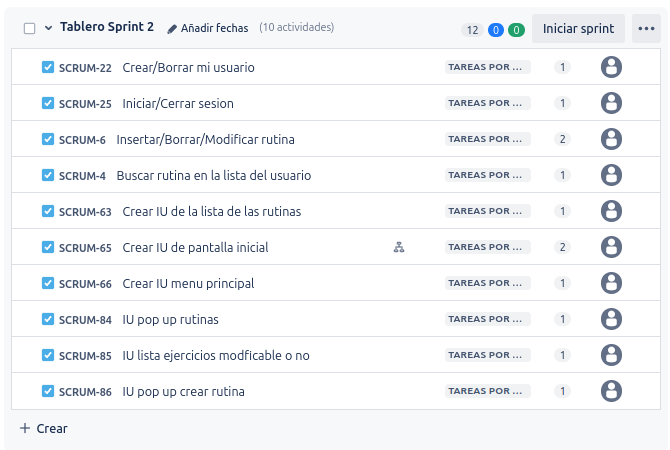
\includegraphics[width=0.7\textwidth]{fotos/PreSprint2.png}
  \caption{Planificaci\'on Sprint 2}
  \label{fig:pre_sprint2}
\end{figure}

\begin{figure}[h!]
  \centering
  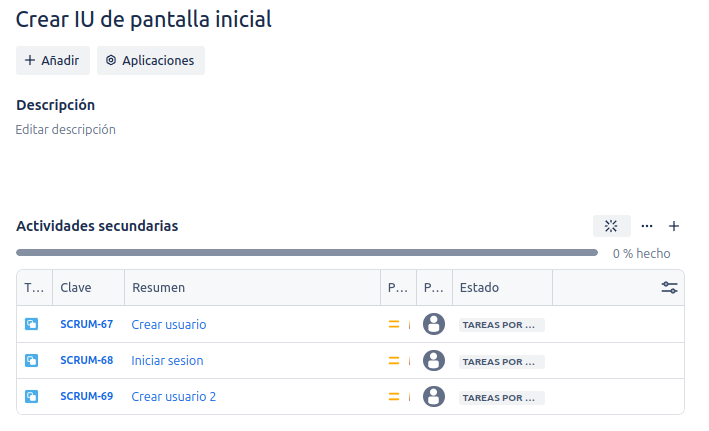
\includegraphics[width=0.7\textwidth]{fotos/SubListPre2.png}
  \caption{Subtareas Sprint 2}
  \label{fig:sublist_pre2}
\end{figure}

\subsubsection*{Sistema de sesiones}
Se implement\'o un sistema de autenticaci\'on basado en tokens. Cuando el usuario verifica su identidad, recibe un token que se guarda en el dispositivo y se usa para validar el acceso posterior. Esto evita que usuarios no autorizados suban contenido haci\'endose pasar por otros.

El backend est\'a desarrollado en \textit{Node.js} y utiliza una base de datos SQL para gestionar las contrase\~nas de los usuarios. Este mismo backend se usar\'a para las funcionalidades de las siguientes iteraciones.

\subsubsection*{API de la app}
La comunicaci\'on entre la app y el servidor se realiza mediante peticiones HTTP. En el futuro, estas podr\'an migrarse a HTTPS para proteger operaciones sensibles. Por ahora se mantiene HTTP para facilitar el depurado.

\subsubsection*{Cambios importantes}
Se redise\~n\'o la implementaci\'on de las pantallas con listas. En lugar de una \'unica clase con condiciones para la visibilidad de elementos, se opt\'o por crear clases espec\'ificas para cada tipo de lista.

\textbf{Ventaja:} El c\'odigo es m\'as limpio, escalable y modular. Si hay que modificar un tipo de lista, los dem\'as no se ven afectados.

\subsubsection*{Sprint Review 2}
Se sugirieron mejoras menores como el ajuste de tama\~nos e iconos en los botones de la secci\'on de creaci\'on de rutinas.

Tambi\'en se modific\'o la funcionalidad de compartir rutinas. Ahora todas son modificables, eliminando la distinci\'on entre rutinas descargadas (antes no modificables) y creadas (modificables). Esto mejora la experiencia del usuario: si desea volver a una rutina original, simplemente la puede volver a buscar y descargar.

\begin{figure}[h!]
  \centering
  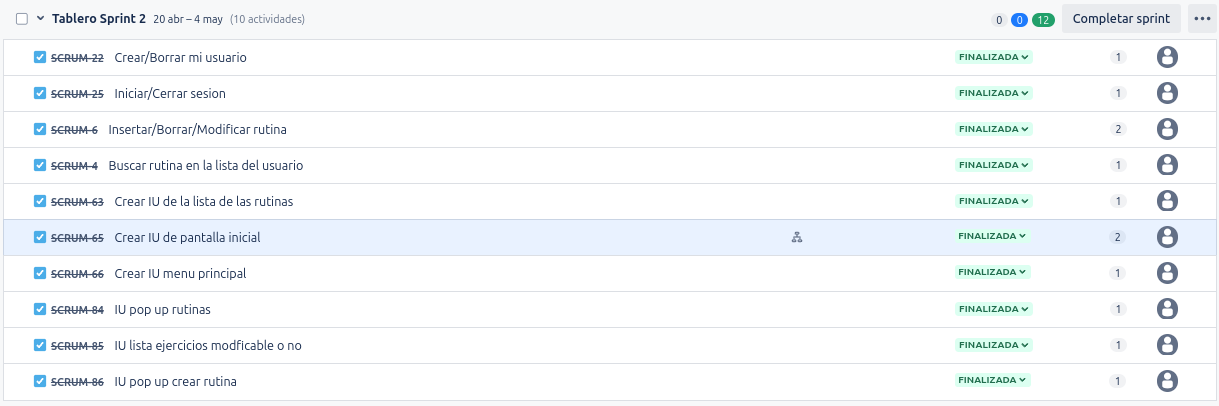
\includegraphics[width=0.7\textwidth]{fotos/PostSprint2.png}
  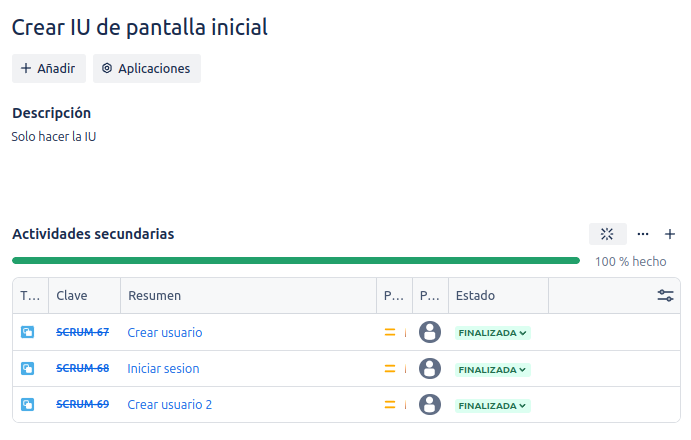
\includegraphics[width=0.7\textwidth]{fotos/SubListPost2.png}
  \caption{Fin Sprint 2 y subtareas}
  \label{fig:post_sprint2}
\end{figure}


\subsection*{Iteraci\'on 3}
Esta iteraci\'on se centr\'o en desarrollar la funcionalidad para compartir rutinas entre usuarios, incluyendo la subida, visualizaci\'on y descarga de rutinas. Adem\'as, se comenz\'o a implementar la funcionalidad de resumen de datos para optimizar el uso de la memoria local.

\begin{figure}[h!]
  \centering
  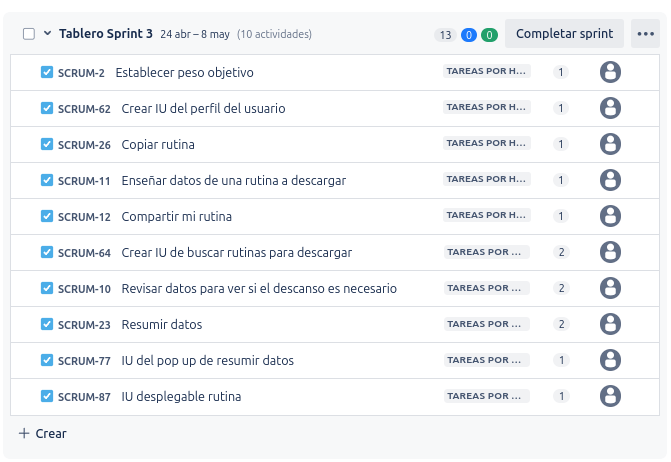
\includegraphics[width=0.7\textwidth]{fotos/PreSprint3.png}
  \caption{Planificaci\'on Sprint 3}
  \label{fig:pre_sprint3}
\end{figure}

\subsubsection*{Peso objetivo}
El peso objetivo es una meta que define el usuario y se almacena en memoria. Esta meta se representar\'a en la gr\'afica de evoluci\'on del peso del usuario, y se generar\'a una alerta cuando dicha meta sea alcanzada. La visualizaci\'on a\'un no ha sido implementada completamente.

\subsubsection*{Cambios durante el desarrollo}
Durante esta iteraci\'on surgieron cambios en la forma de visualizar y gestionar las rutinas compartidas y almacenadas:

\begin{itemize}
  \item Ahora, al descargar una rutina, se a\~nade el nombre del creador al nombre de la rutina, facilitando la distinci\'on entre rutinas propias y descargadas.
  \item Cuando hay conflicto de nombres al crear una rutina, se genera un nombre alternativo del tipo \texttt{Nombre(n)}, siendo \texttt{n} un n\'umero incremental.
  \item Se ha implementado un selector entre ``Mis rutinas'' y ``Compartidas'' para facilitar la visualizaci\'on de las rutinas subidas a la nube por el usuario.
  \item Se reemplaz\'o el filtro integrado en la ventana de b\'usqueda por un selector emergente que permite buscar rutinas por nombre o por nombre de usuario.
  \item La interfaz de descarga y visualizaci\'on de rutinas ahora es un cuadro emergente (pop-up) en lugar de un desplegable.
\end{itemize}

\subsubsection*{Imprevistos y problemas en el desarrollo}
Se identificaron dos errores principales de planificaci\'on:

\begin{description}
  \item[Error 1:] Se planific\'o implementar la funcionalidad de resumir datos sin haber completado la obtenci\'on de datos. \\ \textbf{Soluci\'on:} Replanificar los sprints.
  \item[Error 2:] Se subestim\'o la complejidad del sistema de rutinas compartidas, especialmente en la resoluci\'on de conflictos de nombres. \\ \textbf{Soluci\'on:} Aplicar nombres combinados (nombre + creador + copia) en memoria local e identificadores \textit{autoincrementales} en la nube.
\end{description}

\subsubsection*{Valor a\~nadido a la app}
Los imprevistos y problemas surgidos durante el desarrollo han permitido detectar \textit{bugs}, errores de dise\~no y carencias funcionales que de otro modo podr\'ian haber pasado desapercibidos. Gracias a ello, se han podido proponer nuevas funcionalidades y mejorar las ya existentes, lo cual contribuye significativamente a aumentar la calidad global de la aplicaci\'on.

Algunas de las funcionalidades propuestas como mejora son:

\begin{itemize}
  \item Verificar el token del usuario antes de permitir la subida de rutinas, para evitar plagios.
  \item Al seleccionar la opci\'on de borrar usuario del dispositivo, eliminar tambi\'en la base de datos local asociada.
  \item Crear una base de datos local independiente para cada nuevo usuario creado en un dispositivo.
  \item Posibilidad de editar el nombre de una rutina.
  \item Marcar los ejercicios eliminados con una \textit{flag}, para evitar que se inicien rutinas que los contengan.
  \item Marcar a los usuarios permanentemente eliminados con una \textit{flag}, para proceder a eliminarlos en los dispositvos.
\end{itemize}

Estas funcionalidades est\'an pensadas para aportar mayor \textbf{seguridad}, \textbf{integridad} y \textbf{calidad} al producto final.

\subsubsection{Base de datos del backend}
La base de datos utilizada en el backend está basada en \textit{MySQL}. En ella se almacenan los usuarios junto con sus contraseñas, así como los ejercicios y las rutinas. Las rutinas están vinculadas al usuario que las creó, y los ejercicios se asocian a las rutinas a las que pertenecen. Si un usuario decide eliminar su cuenta de forma permanente, las rutinas y ejercicios relacionados se eliminarán en cascada.

Al descargar una rutina, los ejercicios asociados se guardan en la memoria local del usuario como si fueran de su propiedad. Es decir, el usuario puede modificarlos libremente sin restricciones.

\subsubsection{Sprint Review 3}
